\documentclass[12pt,a4paper]{article}

\usepackage[T1]{fontenc}
\usepackage[utf8]{inputenc}

\usepackage{graphicx}
\graphicspath{ {figures/} }

\usepackage[hidelinks]{hyperref}

\usepackage{csquotes}
\usepackage[UKenglish]{babel}

\usepackage{setspace}
\usepackage{siunitx}
\usepackage{enumitem}
\usepackage[os=win]{menukeys}

\usepackage[margin=3cm]{geometry}


\title{AFM Force Curve Analysis Software Package for Wavemetrics IGOR Pro}
\author{Janne T. Hyotyla}
\date{}


\begin{document}

\maketitle

\setstretch{1.2}

The custom AFM analysis software package consists of IGOR Pro procedure files (WaveMetrics, USA)\footnote{\url{http://www.wavemetrics.com/}}. It has been tested with IGOR version 6.3.4 under Windows 7. The analysis software can be downloaded at \url{https://github.com/jhyot/afm-forcecurve-analysis}.

The software offers a basic user interface for loading force curves and force volume maps from Bruker (formerly Veeco) Nanoscope files, analysing the brush height of each force curve, and reviewing and classifying curves.
Further, additional functionality is available by calling specific functions manually (from the command window, a macro or a procedure).
The software has been tested with data obtained by Nanoscope versions 7.3 and 8.1x.

This manual is divided into three parts. Section~\ref{sec:afmsoftware-config} describes the installation, start and configuration of the software.
Section~\ref{sec:afmsoftware-gui} describes the features accessible through the graphical user interface (GUI), and section~\ref{sec:afmsoftware-functions} finally describes the additional functions not available through the GUI.
Basic familiarity of IGOR Pro operation is assumed, and knowledge about functions and procedures is necessary for using the functions not provided through the GUI.

\section{Installation and configuration}
\label{sec:afmsoftware-config}

\subsection{Installation}
Download the software package and place all included files and folders into any folder. No additional installation is necessary.
In the root folder, \texttt{forcecur\-ve-analysis.ipf} is the main program file. The \texttt{config} folder contains configuration files which can be edited by the user.
The \texttt{lib} folder contains most of the software code, and does not need to be modified by the user.

\subsection{Loading the software}
To load the software package, start Igor by opening the \texttt{forcecurve-analysis.ipf} file (e.g. double-click on the file), or load the file within Igor from the menu \menu{File > Open File > Procedure...}.
Compile the script by selecting \menu{Macros > Compile} from the menu, or \menu{Compile} in the procedure window.
On successful compilation, all the other files are loaded automatically and a new top-level menu entry \menu{Force Map Analysis} will appear (Fig.~\ref{fig:afmsoftware-mainmenu}).

\begin{figure}[htbp]
	\centering
		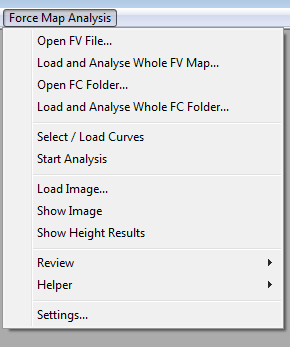
\includegraphics[width=0.5\textwidth]{fig--afmsoftware-mainmenu.png}
	\caption[AFM analysis software menu]{Menu for accessing the GUI functions of the AFM analysis software.}
	\label{fig:afmsoftware-mainmenu}
\end{figure}


\subsection{Configuration}
\label{sec:afmsoftware-configvars}
Some basic parameters for data loading and analysis are configured by editing the file \texttt{config/fca-config.ipf} which is available once the code has been loaded (see above).
Access the file by selecting \menu{Windows > Procedure Windows > fca-config.ipf}. Enable editing by clicking on the pencil symbol in the lower left corner.
This file contains parameters which each control a particular aspect of the software. Change a parameter by editing the part following the assignment symbol \keys{=}.
Parameters have been set to sensible values by default, but depending on the data, changing the values can be necessary for correct results.

The following parameters influence the loading of Nanoscope data files.
\begin{description}[style=nextline]

\item[ksVersionReq]
Lists all valid file versions that can be read by this software (separated by commas). Any files recorded by differing Nanoscope software versions will not be loaded and produce an error to protect from unnoticed wrong loading or analysis. Usually the file format does not change between Nanoscope versions, so additional versions can be added here (see the header of the Nanoscope data file for the version string), but careful inspection of the results should be performed when first loading data from a new version.

\item[ksFixPointNum]
Defines how the number of data points per force curve is determined.\\
\textbf{0}: Automatically read the number of points from the force curve data file.\\
\textbf{1}: Fix the number of points to the value given in the next parameter (this setting is mainly left for legacy reasons).

\item[ksFCPoints]
Number of points per force curve. This parameter only has an effect if \textbf{ksFixPointNum} is set to \textbf{1}.

\item[ksFVRowSize]
Number of pixels per row in a force volume map. Since maps are quadratic, this also defines the number of rows. Only the values \textbf{16} and \textbf{32} have been thoroughly tested.

\item[ksFileTypeFV]
The string by which force volume files are identified (the header of the files is searched for this string). There should be no reason to change this parameter, unless the Nanoscope file format has changed.

\item[ksFileTypeFC]
The string by which single force curve files are identified (the header of the files is searched for this string). There should be no reason to change this parameter, unless the Nanoscope file format has changed.

\item[ksHeaderEnd]
The string which defines the end of the header in data files. There should be no reason to change this parameter, unless the Nanoscope file format has changed.

\end{description}


The following parameters influence aspects of data analysis.
\begin{description}[style=nextline]

\item[ksBaselineFitLength]
Value between 0 and 1. Sets the fraction of the whole force curve length that is used for baseline fitting. Too small values lead to inaccurate fits if the force curve has some irregularities. Too large values also lead to wrong fits if the baseline is not perfectly linear (as can be the case for very long ramp sizes).

\item[ksBrushCutoff]
Used only if the brush height calculation is based on the exponential fit algorithm. Defines the brush height as the distance at which the exponential fit crosses this force value (in \si{pN}). \textbf{Note:} In the current version of the software there is no straightforward way to switch to the exponential fit brush height calculation.

\item[ksBrushOverNoise]
Used only if the brush height calculation is based on the noise threshold algorithm. Defines the brush height as the distance at which the smoothed force curve crosses the smoothed baseline noise multiplied by this factor. Smaller values give larger (more realistic) brush heights but lead to higher susceptibility to noise. Values \num{< 1} are not useful.

\item[ksDeflSens\_ContactLen]
Approximate length of the piezo ramp during which there is contact between tip and sample (in nm). This doesn't have to be accurate but provides guidelines for the fitting algorithm. The default value should work for most force curves. If the deflection sensitivity fit leads to wrong values, changing this parameter can improve results.

\item[ksDeflSens\_EdgeFraction]
Defines how much of the hard-wall portion of a curve is getting fitted for deflection sensitivity. The default value should work for most force curves. If the deflection sensitivity fit leads to wrong values, changing this parameter can improve results. Useful values are in the range of \numrange{0.01}{0.1}.

\item[ksFixDefl]
Defines how the deflection sensitivity is determined for each curve. \textbf{0:} The deflection sensitivity is fitted separately for each curve. \textbf{1:} Read the sensitivity from the header of the force curve or force volume file.

\item[ksXDataZSens]
Defines whether available Z sensor (height sensor) data is used instead of the fixed ideal ramp size set when recording force curves. Using Z sensor gives more correct data. For this, one ramp channel has to be set to Z sensor (sometimes denoted Height sensor) during recording. \textbf{0:} Don't use Z sensor data. \textbf{1:} Use Z sensor data if it is available. \textbf{2:} Always use Z sensor data (aborts data analysis if it is not available).

\item[ksMaxGoodPt]
Some force data may have corrupted data at the end of the curves. If such cases are not detected automatically, this parameter can be set to the point number after which the rest of the force curve is ignored. Set to \textbf{-1} to ignore this parameter.

\end{description}


\section{GUI features}
\label{sec:afmsoftware-gui}

This section describes the features available through the \menu{Force Map Analysis} menu (Fig.~\ref{fig:afmsoftware-mainmenu}).

Before loading and working with a force volume file or a force curve file set, you should create and switch to a new data folder in Igor. Working directly in the root data folder is not recommended. To create a new data folder, select \menu{Data > Data Browser} from the top menu, followed by \menu{New Folder...} in the data browser window.
Enter a unique name and select \menu{Set As Current Data Folder}. Each force curve data set should go into its own data folder. Nested folders are allowed.

\subsection{Loading and analysing data}

\subsubsection{Loading and analysing a force volume file}
Select \menu{Force Map Analysis > Open FV File...}. In the settings dialog, choose whether to load any friction data and Z sensor data present in the FV dataset. Only select yes if your dataset includes this data.
These settings are saved per data folder. If you want to change them later, choose \menu{Settings...} from the menu.
Next, select the file to load. The quasi-topography map appears after successful loading of the FV file.

Choose \menu{Select / Load curves} from the menu to select which force curves from the map to import into Igor and to analyse. Select individual force curves by clicking on the corresponding pixel in the map, or \menu{All} to select all curves.

Next, select \menu{Start Analysis} from the menu to perform the brush height and related analysis of the previously loaded force curves.
After the analysis is finished, an image representing the brush heights is displayed.
Any errors during this step can be related to inappropriate configuration values (see Section~\ref{sec:afmsoftware-configvars}) or trying to load data which is not present (such as Z sensor data).

The menu command \menu{Load and Analyse Whole FV Map...} serves as a shortcut to automatically open a FV file and load and analyse all force curves.

\subsubsection{Navigating through the data}
After successful loading and analysis of the FV data, you can view any force curve by clicking on the corresponding pixel in the quasi-topography or brush height maps. A new graph is shown each time a pixel is selected.
To navigate through the data without opening a new graph, hold \keys{Ctrl} while in the force curve graph and use the arrow keys to navigate around the map.

\begin{figure}[htbp]
	\centering
		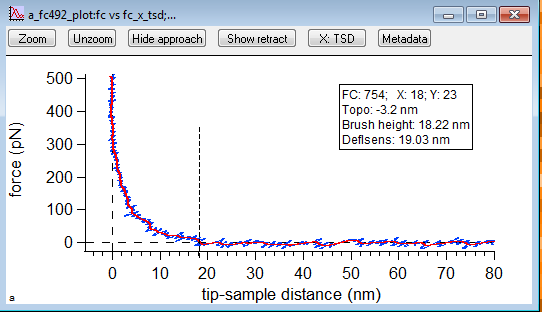
\includegraphics[width=0.7\textwidth]{fig--afmsoftware-fc-graph.png}
	\caption[Force curve graph]{Force curve graph.}
	\label{fig:afmsoftware-fcgraph}
\end{figure}

In the force curve graph (Fig.~\ref{fig:afmsoftware-fcgraph}), you have several buttons to control the data presentation. All regular Igor formatting methods and options are available as well.
The \menu{Zoom} and \menu{Unzoom} buttons cycle through predefined zoom levels. The zoom levels can be re-defined through editing of the source code (see Section~\ref{sec:afmsoftware-zoom}).
The \menu{Approach} and \menu{Retract} buttons show or hide the approach and retract parts of the force curves, respectively.
The button starting with \menu{X: } switches between display modes and displays the current mode. \menu{X: TSD} is showing the force vs tip-sample-distance curve, while \menu{X: Zpiezo} is showing the force vs Z piezo position curve.
\menu{Metadata} prints metadata for the displayed curve gathered during loading and analysing to the command window.

The graphs can be closed at any time, but any changes to the presentation of the graph will be lost.

\subsubsection{Images}
The menu command \menu{Load Image...} allows to select and load a different image as the quasi-topography map. This is useful when you want to process the topography map in a different software (e.g.\ flattening) and then import it back to Igor.
\menu{Show Image} and \menu{Show Height Results} bring the quasi-height image and the brush height map to the front, respectively, if they have been hidden after the initial loading.
Note that closing the images (instead of just hiding them) cannot be undone.

\subsubsection{Loading and analysing a collection of individual force curves}
In addition to a force volume file, this software can also load and analyse individual force curves. Use the menu items \menu{Open FC Folder...}, \menu{Select / Load Curves} and \menu{Start Analysis} (or the shortcut \menu{Load and Analyse Whole FC Folder...}) to import all force curves located in a given folder.
All files in the folder which are recognized as force curves will be analysed. The curve files are imported in the order of their filenames.

After selecting the source folder, you can choose between three different types:

\begin{description}[style=nextline]

\item[line]
Indicates that the individual force curves were taken in a straight line over the surface (e.g.\ using the point-and-shoot mode of Nanoscope).
The cross-section force curve analysis graph will open after the analysis step (Fig.~\ref{fig:afmsoftware-xsectgraph}).

\item[box]
Indicates that the force curves were taken in a quadratic pattern similar to the force volume mode. When selecting this option, the data set behaves as though it was loaded from a force volume file.

\item[random]
Indicates that the force curves have neither a linear nor box-like relation to each other.
After analysis, the cross-section force curve analysis graph will open for ease of analysing and displaying the data. But although the curves are shown to be in one line, this is only for display purposes.

\end{description}

\subsubsection{Cross-section analysis}
The cross-section force curve analysis window (Fig.~\ref{fig:afmsoftware-xsectgraph}) will open after analysis of line or random type force curve data. This window is divided in three parts.
The top part shows the hard-wall topography (black line) and brush height (red area) for each force curve. The middle part shows the force (i.e.\ vertical deflection) data, and the bottom part shows the friction data (horizontal deflection).

The vertical and horizontal deflection graphs show both approach and retract curves. The dashed vertical line indicates the calculated brush contact point.
The buttons above the graph allow to choose between tip-sample-distance and piezo position modes, and to switch between predefined zoom levels.
The zoom levels can be re-defined through editing of the source code (see Section~\ref{sec:afmsoftware-zoom}).
By holding the \keys{Shift} key and moving the mouse over the force curves, a vertical guide appears.
Moving the cross-hair in the top panel (either by dragging it or with left/right arrow keys) selects the corresponding force curve data set.
All graphs can be customized by using the standard Igor features.

\begin{figure}[htbp]
	\centering
		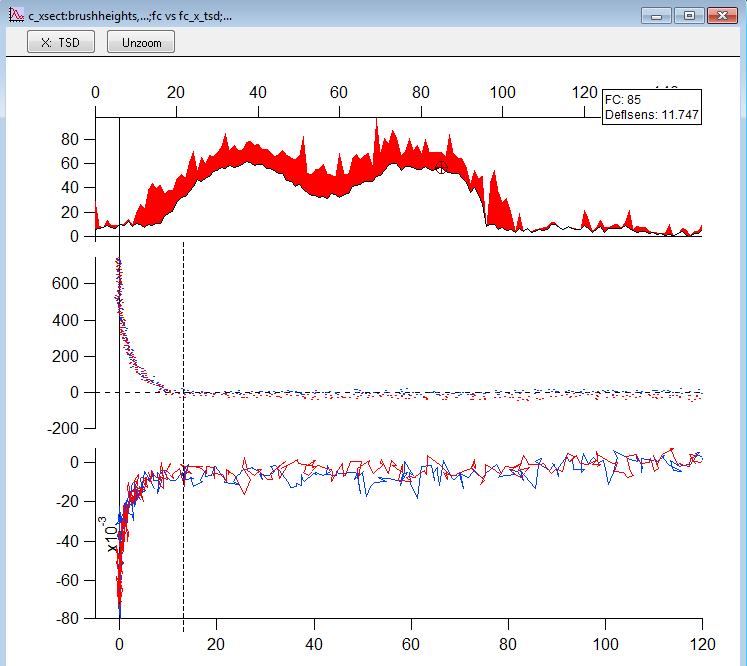
\includegraphics[width=0.9\textwidth]{fig--afmsoftware-xsection-graph.png}
	\caption[Cross-section force curve analysis]{Cross-section force curve analysis window.}
	\label{fig:afmsoftware-xsectgraph}
\end{figure}


\subsection{Reviewing data}
Once data has been loaded and analysed by the software, several data review functions are available through the \menu{Review} submenu.

\subsubsection{Flagging curves}
The function \menu{Review > Flag Curves...} allows to flag force curves based on parametrizable criteria. The different criteria allow to find force curves with general bad quality or incorrect fits.
Once the Flag Curves algorithm has been run, \menu{Review > Mark Flagged} shows the flagged curves as red markers in the topography and brush height images (only for FV data).

The \texttt{flaggedcurves} wave stores the value $1$ at the index of every flagged curve, and can be used for custom analysis or processing of flagged curves.

\subsubsection{Reviewing curves}
Selecting \menu{Review > Review All Curves} or \menu{Review > Review Flagged Curves} starts the review mode. Each curve in turn can be accepted or rejected as a valid data point.
When using \menu{Review Flagged Curves}, the non-flagged curves are automatically accepted as valid.
The \menu{Zoom} and \menu{Unzoom} buttons cycle through the predefined zoom levels (customizable through editing of the source code, see Section~\ref{sec:afmsoftware-zoom}).
The default zoom level for the next curve can be selected in the drop-down list.
The \menu{Redo last} button returns to the previous curve. The \menu{Stop} button stops the review.

Brush heights from accepted and rejected curves are stored in the \texttt{heights\_acc} and \texttt{heights\_rej} waves, respectively. The data can be used to perform calculations and statistical analysis based on the particular subset of data.
If a review is stopped before reviewing all curves, the brush heights from the remaining curves will not be added to either of the new waves.

\subsubsection{Classifying curves}
The \menu{Review > Classify Curves} function is a specialized reviewing tool that was used to analyse the data for Chapter~\ref{sec:escape-transition-geometry}.
In its current form it can only be used to classify force curves taken over a ring-like structure. A force curve can be classified as  \enquote*{exhibiting a certain feature}, or \enquote*{not exhibiting the feature} (or excluded from classification, e.g. when the data quality is too bad).
After the classification step, a histogram is computed that shows the frequency of the classified feature as a function of the distance from the center of the ring (with and without normalizing for the number of curves at a given distance).
Pixels which have low enough quasi-topography height (i.e.\ which lie outside the ring structure) are automatically excluded from classification.

\subsection{Helper Functions}
The \menu{Helper} menu provides access to some utility functions.

\begin{description}[style=nextline]

\item[Brush Histogram]
Calculates and displays a histogram of brush heights over the whole dataset.
The display will not show outliers with very large brush height values, because those are usually measurement or analysis errors.

\item[Subtract Baseline]
Subtracts a baseline (linear fit) from the designated wave. If the active window has a \enquote*{A} cursor placed on a trace, then that wave is used,
otherwise a dialog will ask for the wave name. You can exclude regions from participating in the baseline fit by placing them between pairs of cursors
(i.e.\ between A and B, C and D, etc.). The original wave will be backed up as \path{backups/<wavename>_baselinesubtr}.

\item[Median Filter Image]
Applies a median filter with a $3 \times 3$ pixel kernel to a given image, and also filters out any \texttt{NaN} pixels. You will be asked for the image wave name to be filtered. The original wave will be backed up as \path{backups/<wavename>_medianfilt}.

\end{description}


\section{Additional functions}
\label{sec:afmsoftware-functions}
Some functionality is not accessible via the \menu{Force Map Analysis} menu but only by directly calling specific functions, e.g.\ in the Command Window or from custom scripts.
The following sections briefly describe the additional useful functions, grouped by functionality.
The full explanation of the input and output parameters, and implementation details can be obtained by reading the source code.

\subsection{Brush height analysis}
Most functions in the file \path{lib/fca-analysis.ipf} perform the brush height calculation and related analysis, and are accessible through the menu. Additionally some functions can be called manually for further analysis.
It is recommended to call the additional analysis functions only after performing a regular analysis through the menu, to ensure that all necessary setup is done and waves have been created.

\begin{description}[style=nextline]

\item[CalcLinStiffness]
Calculates the linear brush stiffness for the currently loaded data, as used in section~\ref{sec:brush-stiffness-loading-rate} and described in the Methods in section~\ref{sec:afm-data-analysis}. The resulting data will be saved in the \texttt{linstiffness} wave.

\item[CalcHertzEModAll]
Calculates the brush Young's modulus for the currently loaded data. The algorithm is described in section~\ref{sec:brush-stiffness-loading-rate}. Uses the \texttt{twohertz} curve fitting function from \texttt{lib/fca-fitting.ipf}.
Note that some coefficients for the fit are hardcoded in the \texttt{CalcHertzEMod} function. The calculated $E_1$ and $E_2$ Young's moduli are saved in the \texttt{emod1} and \texttt{emod2} waves.

\end{description}


Functions residing in the file \path{lib/fca-absolute-relative-heights.ipf} are used to produce the \enquote*{brush contact height} analysis and corresponding plots in section~\ref{sec:pegylated-nanoholes}.

\begin{description}[style=nextline]

\item[absrelheights]
Creates the wave that holds the \enquote*{brush contact height} data (i.e. image height plus brush height). It's called \enquote*{absolute} height in the functions, as opposed to \enquote*{relative} height, which is the brush height above the hard-wall contact point.
Parameters \texttt{img} and \texttt{bheights} are existing image and brush height wave names, while the other parameters are names of waves that will be created by the function (absolute brush height wave and the two different \enquote*{zero} lines).

\item[scatterplots]
Creates the scatterplots used in section~\ref{sec:pegylated-nanoholes}. Parameters are as above, with \texttt{img}, \texttt{bheights} and \texttt{added} names of existing waves, while the other two will be created.

\item[plot\_color, plot\_color\_auto]
Creates the coloured areas on the scatterplot (or any other plot). \texttt{plot\_color} takes the color boundary positions as parameters, while \texttt{plot\_color\_auto} chooses the boundaries automatically based on the first $X$ wave data in the plot.

\item[absrelheights\_combine]
Concatenates multiple input waves into a single output wave and displays a scatterplot of the combined data.

\end{description}

\subsection{Loading rate analysis}
The code in \path{lib/fca-loadingrate-analysis.ipf} was used to analyse the data and create the graphs for section~\ref{sec:loadingrate}. Unfortunately, the code is extremely specialised for the particular task and no effort has been spent to make it more general and user-friendly.
The interested reader is welcome to look through the code and associated comments.


\subsection{Helper Functions}
Helper functions assist with miscellaneous small tasks. The functions are located in \path{lib/fca-datainfo.ipf} and \path{lib/fca-wave-handling.ipf}.

\begin{description}[style=nextline]

\item[PrintInfo, PrintInfoDF]
Prints information about the current data folder or one passed as parameter.

\item[PrintParams]
Prints analysis and curve parameters. The desired parameters must be passed into the function. The function searches global analysis parameters and per-curve parameters and prints out any matches. The second input argument selects the curve number for which to print the parameters.
To see what parameters are available, have a look at the \path{internalvars/analysisparameters} variable and at the \texttt{fcmeta} text wave.

\item[SaveBackupWave, RestoreBackupWave]
Saves and restores a given wave to/from the \texttt{backups} data folder.

\item[MakeTempCurve]
Extracts a single curve from the full curve dataset. This can be used to try out analysis and operations on a given wave. It is intended to be used with the \texttt{fc} and \texttt{rfc} group of 2D waves.
The index to be extracted can be passed in by hand or it can be read from an open graph displaying the desired curve.

\end{description}

\subsection{Curve Fitting}
The curve fitting functions in \path{lib/fca-fitting.ipf} can be used from a script or from the Igor \menu{Analysis > Curve Fitting...} dialog. The mathematical formulas can be found in the code comments within the individual functions.
Most functions are transformed to work with \si{nm} and \si{pN} units, since the loaded and analysed force curves are saved in these units.


\subsection{Zoom settings}
\label{sec:afmsoftware-zoom}
Although all graphs can use standard Igor zooming and scaling functions, many force curve graphs include special zoom buttons for convenient setting of standard zoom levels.
The zoom levels can be configured in the \path{config/fca-zoom-config.ipf} file.
The configuration is done by editing a matrix with zoom values. Each field in the matrix corresponds to a curve type, zoom level, and axis.
The source file has additional comments to help with finding the correct field for changing a specific zoom setting.


\end{document}  